\icode[magenta]{E-ME-MU-L4-261019-003}
轻质细线绕过两个等高、光滑定滑轮\(P\)、\(Q\)，两端分别连接着质量均为\(m\)的小球\(A\)、\(B\)，已知\(P\)、\(Q\)间细线水平，间距为\(l\)，\(A\)、\(B\)小球处于静止状态。现将一质量也为\(m\)的物体\(C\)，通过光滑的轻挂钩挂在细线上与两定滑轮等间距的位置\(O\)，静止释放后向下运动。若\(A\)、\(B\)始终没有与\(P\)、\(Q\)相碰，重力加速度为\(g\)，则\(C\)物体在下降过程中\paren[]
	
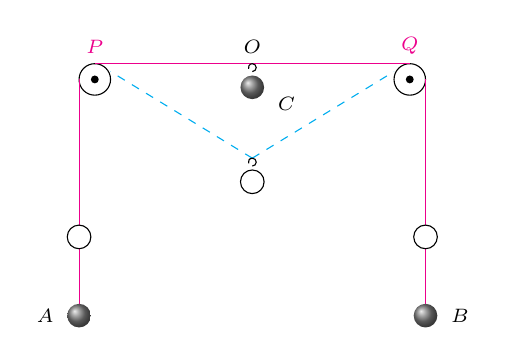
\begin{tikzpicture}[font=\scriptsize]
	\draw (-2,0) circle(.2) (2,0) circle(.2);
	\fill (-2,0) circle(.05) (2,0) circle(.05);
	\draw[magenta] (-2,.2)node[above]{\(P\)}--(2,.2)node[above]{\(Q\)} (-2.2,0)--(-2.2,-3) (2.2,0)--(2.2,-3);
	\shade[ball color=gray] (-2.2,-3) circle(.15);
	\shade[ball color=gray] (2.2,-3) circle(.15);
	\shade[ball color=gray] (0,-.1) circle(.15);
	\draw[yshift=.2cm] (0,-.1) arc(-90:200:.05);
	\draw[dashed,cyan] (0,-1)--(-1.8,0.1) (0,-1)--(1.8,0.1);
	\draw[yshift=-1cm] (0,-.1) arc(-90:200:.05);
	\draw[fill=white] (0,-1.3)circle(.15);
	\draw[fill=white] (-2.2,-2) circle(.15);
	\draw[fill=white] (2.2,-2) circle(.15);
	\node at(-2.4,-3)[left]{\(A\)};
	\node at(2.4,-3)[right]{\(B\)};
	\node at(0,.2)[above]{\(O\)};
	\node at(.2,-.1)[below right]{\(C\)};
\end{tikzpicture}
\begin{choices}
	\item 速度先增大后减小
	\item 加速度先增大后减小
	\item 最大动能为\(\frac{2 - \sqrt{3}}{2}mgl\)
	\item 下降最大高度为\(\frac{2l}{3}\)
\end{choices}
\begin{answer}
    
\end{answer}